\usetikzlibrary{angles,quotes}
\begin{question}
\noindent Two space observatories, $A$ and $B$, are tracking a satellite, $S$, as it passes overhead. Observatory $B$ is due east of Observatory $A$.

\noindent The bearing of the satellite $S$ from Observatory $A$ is $065^\circ$.\\
The bearing of the satellite $S$ from Observatory $B$ is $312^\circ$.

\begin{center}
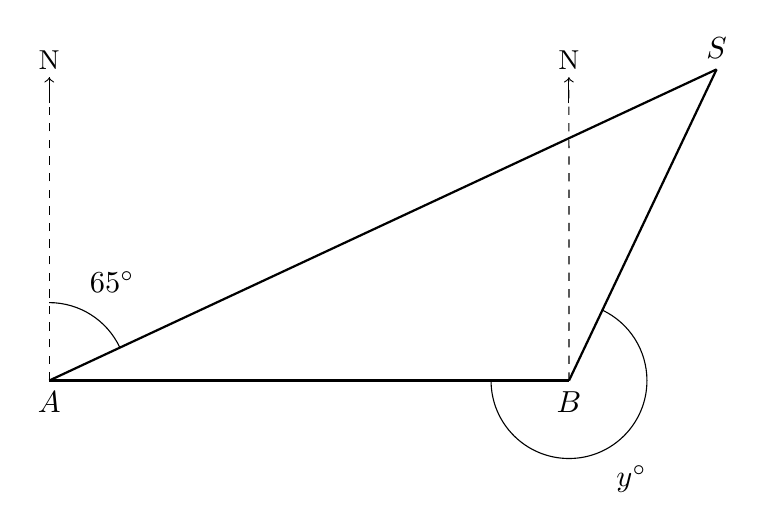
\begin{tikzpicture}[scale=1.1, transform shape]
    \coordinate (A) at (0,0);
    \coordinate (B) at (6,0);
    % S is placed so that bearing from A is 65 degrees (i.e. 25 degrees above the horizontal AB line)
    \coordinate (S) at (25:8.5);

    % East-West line through A and B
    \draw[thick] (A) -- (B);
    \node[below] at (A) {$A$};
    \node[below] at (B) {$B$};

    % North lines (dashed, parallel) at A and B
    \draw[dashed] (A) -- (0,3.5);
    \draw[->] (0,3.2) -- (0,3.5);
    \node[font=\small] at (0,3.7) {N};

    \draw[dashed] (B) -- (6,3.5);
    \draw[->] (6,3.2) -- (6,3.5);
    \node[font=\small] at (6,3.7) {N};

    \coordinate (JA) at (0,3.5);
    \coordinate (JB) at (6,3.5);

    % Lines from A and B to S
    \draw[thick] (A) -- (S);
    \draw[thick] (B) -- (S);
    \node[above] at (S) {$S$};

    % Bearing angle at A (from North, clockwise to S) = 65 degrees
    \pic [draw, angle radius=0.9cm, "$65^\circ$", angle eccentricity=1.5] {angle = S--A--JA};

    % Angle at B between North (pointing up) and BA (pointing to A, i.e. west) - the reflex bearing 312 means angle from North clockwise back round to S is 312, so angle from North to S going anticlockwise (i.e. westward first) is 360-312=48 degrees on the west side. We mark angle between BA (west direction) and BS.
    \pic [draw, angle radius=0.9cm, "$y^\circ$", angle eccentricity=1.5] {angle = A--B--S};

\end{tikzpicture}
\end{center}

\noindent (a) Show that the angle marked $y^\circ$ in the diagram, angle $ABS$, is $42^\circ$.

\vspace{4cm}
\answermarks{2}

\noindent (b) Hence, using angle facts for the parallel North lines at $A$ and $B$, work out the bearing of Observatory $A$ from the satellite $S$.

\vspace{4cm}
\answerequnit{}{$^\circ$}{2}
\end{question}
